\section{Parallelizzazione}
\label{sec:parallelization}
Come gi\`a detto rappresentiamo il gioco della vita con una matrice. Siccome l'algoritmo prevede di computare ogni cella della matrice, il modo pi\`u opportuno per parallelizzare e ditribuire il calcolo \`e suddividere la matrice in \textbf{fette} ed assegnare una fetta ad ogni \textbf{PE} (Process Element)\footnote{Process Element: pu\`o essere un processo concorrente su una singola macchina oppure una macchina dedicata al calcolo.} che gli potr\`a applicare l'algoritmo in modo parallelo.
\begin{figure}[ht]
  \centering
  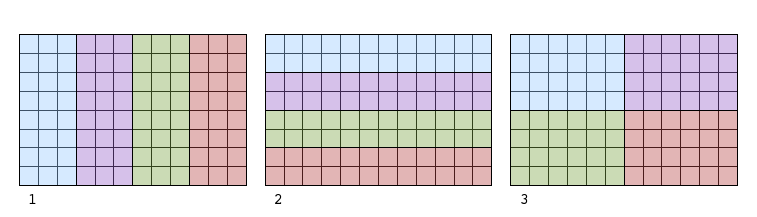
\includegraphics[width=\columnwidth]{matrix-division.png}
  \caption{\emph{Suddivisione della matrice in fette: per colonne (1), per righe (2) o per ``pezzi'' (3).}}
  \label{fig:matrix_division}
\end{figure}
Nella figura \ref{fig:matrix_division} sono rappresentate tre tipi di suddivisioni: per colonne, per righe e per ``pezzi''. La suddivisione influisce sulle prestazioni poich\'e, come si vedr\`a meglio pi\`u avanti, ogni PE che ha una fetta dovr\`a comunicare (in una fase di sincronizzazione) con i PE che hanno le fette di matrice confinanti alla sua. Allora le prime due suddivisioni praticamente si equivalgono (nel caso di matrici quadrate sarebbero identiche, altrimenti dipende se ci sono pi\`u righe o colonne), mentre la terza, per ``pezzi'', non porta alcun vantaggio rispetto alle prime due, ma anzi pu\`o portare alcuni problemi dato che ogni fetta confina con altre otto fette (tenendo sempre conto della regola che il mondo gira attorno), mentre con le prime due si ha che ogni fetta confina solamente con altre due fette. Perci\`o la matrice verr\`a suddivisa per colonne, assegnando quindi ad ogni PE un certo numero di colonne della matrice, su cui poi eseguir\`a l'algoritmo del gioco della vita. Siccome suddividiamo la matrice per colonne, chiameremo \textbf{bordo sinistro} della fetta la prima colonna e \textbf{bordo destro} l'ultima colonna della fetta, ovvero l'insieme delle celle che hanno come vicini celle in altre fette. Chiameremo inoltre \textbf{vicino destro} di un PE il PE che ha la fetta precedente alla sua, mentre il \textbf{vicino sinistro} sar\`a il PE che ha la fetta successiva. Da notare che non necessariamente due PE con indice consecutivo, ad esempio il PE 0 e il PE 1, saranno vicini, ma dipender\`a da quale fetta gli verr\`a assegnata.

Ogni PE, per applicare l'algoritmo del gioco della vita sulla propria fetta, calcola il valore di una cella sulla base delle otto celle vicine; se ogni PE vede per\`o solamente la sua fetta non riuscir\`a mai a calcolare neanche una singola iterazione siccome non conosce i valori delle celle vicine alle celle sui bordi, che fanno parte di una fetta assegnata ad un'altro PE. Si deve quindi dare in qualche modo, ad ogni PE, una visione dei bordi dei PE vicini.

Una prima soluzione pu\`o essere dare una copia dell'intera matrice ad ogni PE, con un approccio fortemente centralizzato, in cui ogni PE pu\`o comunicare solamente con un PE radice; il processo potrebbe seguire quindi i seguenti passi:
\begin{enumerate}
  \item Il PE radice comunica a tutti i PE la matrice completa e la fetta di cui ognuno si deve occupare.
  \item Ogni PE compie un'iterazione sulle celle della fetta che gli \`e stata assegnata, guardando i vicini delle celle nella propria copia locale della matrice.
  \item Terminata un'iterazione, ogni PE rimanda indietro alla radice solamente la fetta di matrice che ha modificato.
  \item La radice riceve tutte le fette e ricostruisce la matrice, che a questo punto rappresenta la generazione successiva, e ricomincia il processo dall'inizio fino a compiere \textit{n} iterazoni.
\end{enumerate}
Seppur corretto e funzionante, questo approccio ha l'evidente problema che viene perso molto tempo per trasferire dati inutili. Infatti ogni PE riceve l'intera matrice all'inizio di ogni iterazione, quando gli basterebbe ricevere solamente la sua fetta pi\`u le due colonne dei bordi dei PE vicini, mentre il PE radice riceve l'intera matrice alla fine di ogni iterazione. Se indichiamo con con \textit{p} il numero di PE coinvolti, in totale vengono trasferite \textit{p} matrici ad ogni iterazione; considerando che la matirce sar\`a di notevoli dimensioni (migliaia di righe per migliaia di colonne) con questo apporccio si rischia di perdere pi\`u tempo a trasferire dati che ad eseguire l'algoritmo.

Come detto, ad ogni PE che deve eseguire l'algoritmo gli basta ricevere la fetta su cui deve lavorare pi\`u le due colonne dei PE vicini. Ma ovviamente ad ogni iterazione le colonne dei PE vicini devono essere aggiornate perch\'e anche su quelle colonne \`e passata una generazione. Rimanendo nell'approccio precedente ogni PE potrebbe ricevere la fetta pi\`u le due colonne, eseguire un'iterazione sulla sua fetta, rimandarla al PE radice il quale ricostruisce la matrice e rinvia le fette e le colonne aggiornate ad ogni PE, ricominciando l'intero processo. \`E per\`o subito evidente che il processo pu\`o essere ulteriormente migliorato facendo in modo che ogni PE scambi direttamente i suoi bordi con i PE vicini, senza passare da un PE centralizzato, che porterebbe ad un rallentamento del calcolo. Allora si pu\`o migliorare l'approccio precedente nel modo seguente:
\begin{figure}[ht]
  \centering
  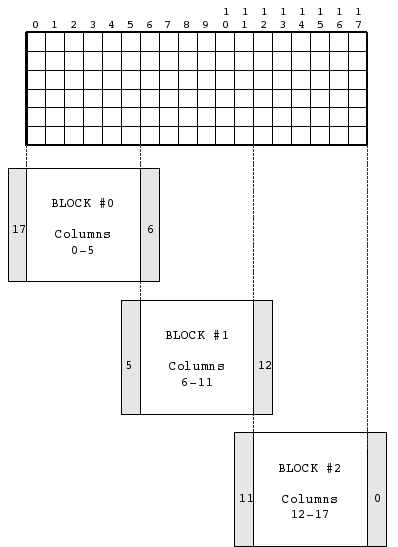
\includegraphics[width=0.7\columnwidth]{matrix-blocks.png}
  \caption{\emph{Suddivisione di una matrice 6x18 in 3 blocchi.}}
  \label{fig:matrix_blocks}
\end{figure}
\begin{enumerate}
  \item Il PE radice costruisce la matrice e e la suddivide in \textbf{blocchi}, composti dalla fetta di matrice su cui un PE lavorer\`a, pi\`u la colonna immediatamente a sinistra prima della fetta ed immediatamente a destra dopo la fetta, che serviranno al PE per calcolare i valori delle celle nel bordo della sua fetta; dopodich\'e invia un blocco ad ogni PE. Nella figura \ref{fig:matrix_blocks} si pu\`o vedere un esempio di come la matrice viene separata in blocchi. Ogni blocco \`e composto da una fetta di matrice pi\`u due vettori, che chiameremo \textbf{vettore sinistro} e \textbf{vettore destro}, che rappresentano rispettivamente il bordo destro del blocco a sinistra e il bordo sinistro del blocco a destra.
  \item I PE eseguono un'iterazione sulla loro fetta di matrice, utilizzando i vettori del blocco per calcolare i nuovi valori delle celle sul bordo.
  \item Ogni PE si sincronizza con gli altri aspettando che tutti abbiano concluso l'iterazione.
  \item Ogni PE invia il suo bordo destro al vicino destro ed il suo bordo sinistro al suo vicino sinistro, aspettandosi di ricevere i rispettivi bordi dai rispettivi vicini che andranno ad aggiornare i vettori del blocco. A questo punto ogni PE ha i vettori aggiornati e pu\`o procedere ad un'altra iterazione.
  \item Quando un PE ha eseguito \textit{n} iterazioni sul suo blocco, lo rinvia al PE radice che ricostruisce la matrice che sar\`a il risultato del gioco della vita.
\end{enumerate}
Con questo approccio si riesce a ridurre al minimo la quantit\`a di dati scambiati tra i processi ed in questo modo si potranno ottenere prestazioni ottimali dalla parallelizzazione. Questo metodo \`e quello che verr\`a utilizzato nell'implementazione parallela del gioco della vita, e pi\`u avanti vengono descritti i dettagli su come dividere esattamente la matrice e come si possono sincronizzare i PE alla fine di ogni iterazione.

Un altro modo possibile per risolvere il problema delle celle sui bordi \`e un approccio ``su richiesta''. Invece che scambiarsi ad ogni iterazione le intere colonne dei bordi, ogni PE potrebbe fare la richiesta del valore della cella che non fa parte della sua fetta direttamente al PE vicino nel momento in cui gli serve (quindi durante il calcolo dell'iterazione). In questo modo si riuscirebbero ad ottenere benefici se solo alcune delle celle nei bordi fossero elaborate, poich\'e in tal caso non sarebbe necessario scambiarsi l'intera colonna ma sarebbero sufficienti solo pochi valori relativi ad alcune celle. Siccome per\`o l'alogritmo prevede di elaborare tutte le celle, due processi si dovrebbero comunque comunicare l'intera colonna, in questo caso non tutta in una volta ma un valore alla volta, quando richiesto, portando per\`o a rallentamenti dovuti alle numerose operazioni di sincronizzazione che sarebbero necessarie per scambiarsi i valori in questo modo. Per questo si preferisce utilizzare l'approccio precedente, in cui \`e necessaria una sola operazione di sincronizzazione alla fine di ogni iterazione.

\subsection{Bilanciamento del carico di lavoro}
Stabilito che per il calcolo parallelo la matrice viene suddivisa per colonne, e ad ogni PE verranno quindi assegnate un certo numero di colonne su cui dovr\`a lavorare, resta da specificare come esattamente dividere la matrice dato il numero di PE, ovvero quante colonne mettere in ogni blocco.

Diciamo allora che abbiamo una matrice di \textit{c} colonne (il numero di righe \`e ininfluente), ed \textit{n} PE a cui poter assegnare dei blocchi di matrice su cui lavorare. Assumiamo che \textit{n} sia minore-uguale a \textit{c} (il caso in cui \textit{n} \`e maggiore non ha senso dal lato pratico, percui lo escludiamo). Naturalmente se \textit{n} divide esattamente \textit{c} (senza resto), allora daremo \textit{c}/\textit{n} colonne ad ogni PE, in questo modo ogni PE avr\`a lo stesso carico di lavoro. Se invece \textit{n} non divide \textit{c}, si potrebbe pensare di assegnare il resto della divisione all'ultimo PE (in aggiunta alle altre colonne gi\`a assegnate); quindi, per esempio, se abbiamo una matrice 32x32 e 6 PE, assegnamo 5 colonne ai PE da 0 a 4, e 7 colonne (5 + il resto 2) al PE numero 5. In questo modo un PE si troverebbe con pi\`u lavoro da eseguire rispetto agli altri, e questa non \`e solo un'ingiustizia, ma porterebbe anche ad un rallentamento degli altri PE. Infatti alla fine di ogni iterazione \`e previsto che ogni PE si sincronizzi con gli altri per scambiarsi il proprio bordo, e se un solo PE tarda rallenta anche l'esecuzione degli altri. Percui, in generale, un buon assegnamento delle colonne ai PE influisce sulle prestazioni dell'intero processo, come rappresentato in figura \ref{fig:imbalanced_columns}.
\begin{figure}[ht]
  \centering
  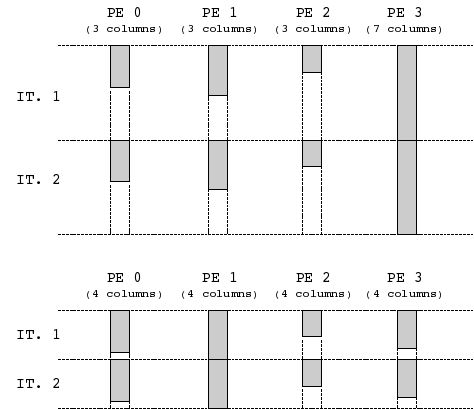
\includegraphics[width=0.7\columnwidth]{imbalanced-columns.png}
  \caption{\emph{Un bilanciamento sbagliato delle colonne pu\`o avere forti ripercussioni sul tempo totale di esecuzione.}}
  \label{fig:imbalanced_columns}
\end{figure}

Allora l'ideale \`e avere una situazione in cui ogni PE ha ``praticamente'' lo stesso numero di colonne degli altri. Il problema si pone quando vi \`e del resto nella divisione tra il numero di colonne \textit{c} e il numero di PE \textit{n}. Allora, intuitivamente, si pu\`o assegnare uno stesso numero di colonne ad ogni PE ($ \lfloor c/n \rfloor $) e distribuire un eventuale resto \textit{r} assegnando una sola colonna in pi\`u ai primi \textit{r} PE, poich\`e sicuramente si ha \textit{r} < \textit{n}. In altre parole l'idea \`e di assegnare ciclicamente una colonna per volta ad ogni PE, se in questo modo l'ultima colonna viene assegnata all'ultimo PE significa che non c'era resto, altrimenti i primi \textit{r} PE avranno una colonna in pi\`u rispetto agli altri. Con questo metodo si ottiene una situazione in cui, per qualunque numero di colonne, ogni PE avr\`a al pi\`u una colonna in pi\`u rispetto agli altri PE; considerando che, in casi reali, ogni PE avr\`a centinaia di colonne da processare, una in pi\`u non appesantisce in modo rilevante il carico di lavoro.

Ovviamente si deve assegnare ad ogni PE un blocco della matrice con un certo numero di colonne consecutive, percui si vuol sapere, al momento della suddivisione in blocchi, il numero di colonne che ogni blocco deve avere. Dato \texttt{C} il numero di colonne della matrice, \texttt{N} il numero di blocchi in cui si vuole suddividere la matrice (che sar\`a il numero di PE che devono ricevere un blocco) ed \texttt{I} il numero del blocco che si vuole costruire, il seguente algoritmo restituisce il numero di colonne da assegnare al blocco in accordo con il metodo appena descritto:
\begin{verbatim}
number_of_columns(C, N, I) {
  D := parte_intera_inferiore(C/N);
  R := C mod N;
  if I < R then
    return D + 1;
  else
    return D;
}
\end{verbatim}
Come gi\`a detto, utilizzando questo algoritmo, si pu\`o separare la matrice in blocchi che differiscono al pi\`u di una colonna, ottenendo cos\`i un ottimo bilanciamento del carico di lavoro dei PE che dovranno applicare il gioco della vita sui blocchi.

\subsection{Sincronizzazione}
Alla fine di ogni iterazione ogni PE deve scambiare i propri bordi con i PE vicini ed aggiornare i vettori del suo blocco ricevendo i bordi dei vicini. Un esempio degli scambi che devono avvenire si pu\`o vedere in figura \ref{fig:boundary_exchange}.
\begin{figure}[ht]
  \centering
  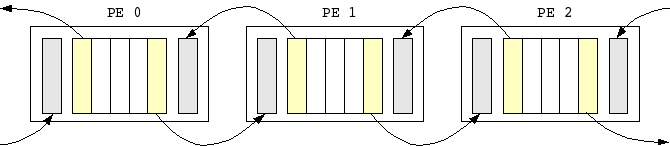
\includegraphics[width=0.9\columnwidth]{boundary-exchange.png}
  \caption{\emph{Lo scambio dei bordi tra PE alla fine di ogni iterazione. Ogni PE ha il suo blocco su cui ha eseguito un'iterazione, composto dalla fetta di matrice (con evidenziate le colonne di bordo) e dai due vettori sinistro e destro che devono essere aggiornati.}}
  \label{fig:boundary_exchange}
\end{figure}

Guardando la figura si pu\`o capire quanto sia delicato questo passaggio e che pu\`o essere molto facile arrivare ad un deadlock in questa fase di sincronizzazione. Assumiamo allora di avere una funzione \textit{send} non bloccante per spedire una colonna del blocco e una funzione \textit{receive} bloccante per ricevere una colonna. Un primo modo per sincronizzare i dati tra i PE pu\`o essere un modello a catena come quello raffigurato in figura \ref{fig:pe_synchronization_1}.
\begin{figure}[ht]
  \centering
  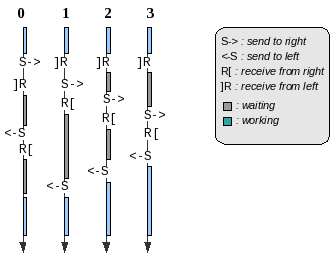
\includegraphics[width=0.6\columnwidth]{pe-synchronization-1.png}
  \caption{\emph{Un esempio del primo approccio alla sincronizzazione, con 4 PE.}}
  \label{fig:pe_synchronization_1}
\end{figure}

Tutti i PE tranne quello con il primo blocco si mettono in attesa di ricevere il vettore sinistro, mentre il PE con il primo blocco \`e il primo ad inviare il suo bordo destro al vicino destro, dopodich\'e si mette in attesa di ricevere dal vicino sinistro. Mano a mano che un PE finisce di ricevere il suo vettore sinistro, spedisce il bordo destro al vicino a destra, e si rimette in attesa per ricevere il vettore destro dal vicino destro. Il primo ciclo si chiude quando il PE che ha l'ultimo blocco spedisce il suo bordo destro al PE iniziale, a questo punto la catena si inverte e il primo PE spedisce all'ultimo PE il suo bordo sinistro e si mette in attesa di ricevere dal vicino destro. Ricomincia quindi il ciclo inverso, che si conclude con il primo processo che riceve il vettore destro dal vicino destro. \`E facile vedere che con questo semplice approccio non si potranno mai creare deadlock, inoltre pu\`o andare bene per un qualunque numero di PE (maggiore-uguale a 2). \`E per\`o altrettanto evidente che viene sprecato molto tempo per scambiarsi i dati in questa catena in cui nessun PE (a parte il primo) spedisce prima di aver ricevuto, che porta ad uno scambio di dati che si potrebbe definire sequenziale, mentre sarebbe intuitivamente possibilie scambiarsi i dati in modo parallelo, cio\`e mentre due PE stanno trasmettendo tra loro, altri due potrebbero contemporaneamente fare lo stesso, e risparmiare quindi nel tempo totale della sincronizzazione.

Per effettuare uno scambio di dati parallelo adottiamo allora uno schema differenta, che chiameremo pari-dispari, in cui i PE eseguiranno passi diversi a seconda se hanno un blocco pari (blocco numero 0, 2, 4, ecc.) o dispari (blocco numero 1, 3, 5, ecc.):
\begin{itemize}
  \item PE con blocco pari.
    \begin{enumerate}
      \item Spedisce il bordo destro al vicino destro.
      \item Riceve il vettore sinistro dal vicino sinistro.
      \item Spedisce il bordo sinistro al vicino sinistro.
      \item Riceve il vettore destro dal vicino destro.
    \end{enumerate}
  \item PE con blocco dispari.
    \begin{enumerate}
      \item Riceve il vettore sinistro dal vicino sinistro.
      \item Spedisce il bordo destro al vicino destro.
      \item Riceve il vettore destro dal vicino destro.
      \item Spedisce il bordo sinistro al vicino sinistro.
    \end{enumerate}
\end{itemize}
Dopodich\'e ovviamente ogni PE pu\`o eseguire l'iterazione successiva sul suo blocco. In figura \ref{fig:pe_synchronization_2} si pu\`o vedere un esempio con un numero pari e dispari di blocchi. Per leggere a modo la figura bisogna sempre tenere conto che ``il mondo gira attorno'', percui l'ultimo blocco comunica con il primo blocco, e viceversa, e che le send sono operazioni non bloccanti mentre le receive sono operazioni bloccanti e possono leggere una send anche dopo che \`e stata inviata (si pu\`o pensare che il messaggio venga memorizzato in un buffer locale al PE che lo ha ricevuto, il quale pu\`o anche andare a prenderlo in un secondo momento).
\begin{figure}[ht]
  \centering
  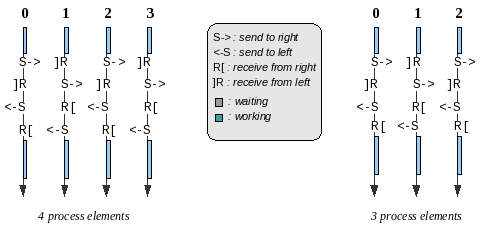
\includegraphics[width=0.9\columnwidth]{pe-synchronization-2.png}
  \caption{\emph{Esempio di sincronizzazione pari-dispari con 4 e 3 PE.}}
  \label{fig:pe_synchronization_2}
\end{figure}
Ovviamente le cose possono non andare perfettamente come rappresentate in figura, un PE pu\`o impiegare pi\`u tempo degli altri ad arrivare alla fase di sincronizzazione (ed in pratica si avr\`a sempre una situazione in cui ogni PE arriver\`a in tempi diversi), ma questo non comporta problemi, assumendo che non possano esserci errori ed ogni \textit{send} e \textit{receive} vada sempre a buon fine, infatti si ha solamente un rallentamento dei PE vicini, che si mettono in attesa di ricevere i messaggi del PE in ritardo, situazione comunque inevitabile siccome ad ogni iterazione \`e necessaria una sincronizzazione che dipende dal calcolo di altri PE.

Quindi, con questo tipo di sincronizzazione, si ha la possibilit\`a di scambiare i dati in parallelo, senza deadlock, e sia per un numero pari di processi che per un numero dispari. Inoltre non sono necessarie barriere alla fine della sincronizzazione, infatti un PE prosegue con l'iterazione \textit{k+1} solamente se ha inviato i suoi bordi e ricevuto i vettori dell'iterazione \textit{k}, percui se un PE \`e riuscito ad aggiornare i suoi due vettori pu\`o proseguire con l'iterazione successiva senza attendere oltre.

Per i vantaggi portati e per la semplicit\`a della procedura verr\`a utilizzato questo approccio (pari-dispari) per la sincronizzazione dei bordi fra i PE.

\subsection{Lo skeleton: una farm}
Lo schema descritto fin'ora consiste in un PE iniziale che suddivide la matrice in blocchi in base a quanti altri PE sono disponibili ad elaborarli, dopodich\'e invia ad ogni PE un blocco su cui verranno eseguite le \textit{n} iterazioni dell'algoritmo del gioco della vita; i PE che elaborano i blocchi si sincronizzano ad ogni iterazione, per poi spedire, compute le \textit{n} iterazioni, i blocchi elaborati ad un PE finale che riassembla la matrice e restituisce il risultato finale dell'intero processo.
\begin{figure}[ht]
  \centering
  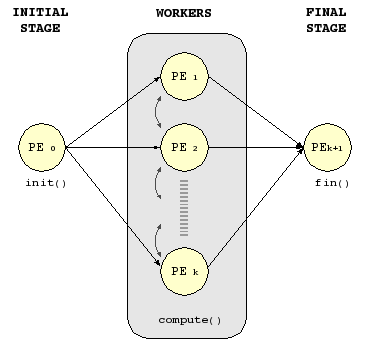
\includegraphics[width=0.7\columnwidth]{farm.png}
  \caption{\emph{Una Farm con \textit{k} workers.}}
  \label{fig:farm}
\end{figure}

Questo schema pu\`o essere implementato con una \textbf{Farm}, in figura \ref{fig:farm}, composta da un PE iniziale (\textbf{initial stage}), un insieme di PE che chiameremo \textbf{workers} che lavorano in parallelo, ed un PE finale (\textbf{final stage}). Lo stage iniziale costruisce una serie di blocchi a partire dalla matrice iniziale (funzione \texttt{init()}) e li spedisce ai workers che li elaborano applicandogli \textit{n} iterazioni dell'algoritmo del gioco della vita (\texttt{compute()}), in modo parallelo l'uno con l'altro, e sincronizzandosi ad ogni iterazione; infine i workers inviano i blocchi elaborati allo stage finale che li raccoglie e ricostruisce la matrice (\texttt{fin()}) che sar\`a il risultato dell'intero processo.
